\documentclass[a4paper,french]{article}
%\usepackage[T1]{fontenc}		% la font bien
\usepackage[utf8]{inputenc}		% les accents
\usepackage[french]{babel}		% la langue
\usepackage{amsmath,amssymb}	% math
\usepackage{graphicx,color,import,float,subcaption}  % graph
\usepackage[margin=2cm]{geometry} % marges
\usepackage{multicol,multirow}	% tables
\usepackage{todonotes}			% penses-bêtes
\usepackage{wrapfig}			% figures sur le côté
\usepackage{hyperref}			% liens vers les figures et formules
\usepackage{lipsum, comment}

\renewcommand{\thesubfigure}{\roman{subfigure}} % Numérotation romaine des sous-figures pour éviter collision avec légende

\begin{document}

\title{\textsc{Cristaux de glace}}
\date{\today}
\maketitle

\section*{But}
	Observer différentes formes de cristaux de glaces.

\section*{Montage}
	\begin{figure}[h]
		\centering
		\begin{subfigure}[b]{0.54\textwidth}
		\centering
		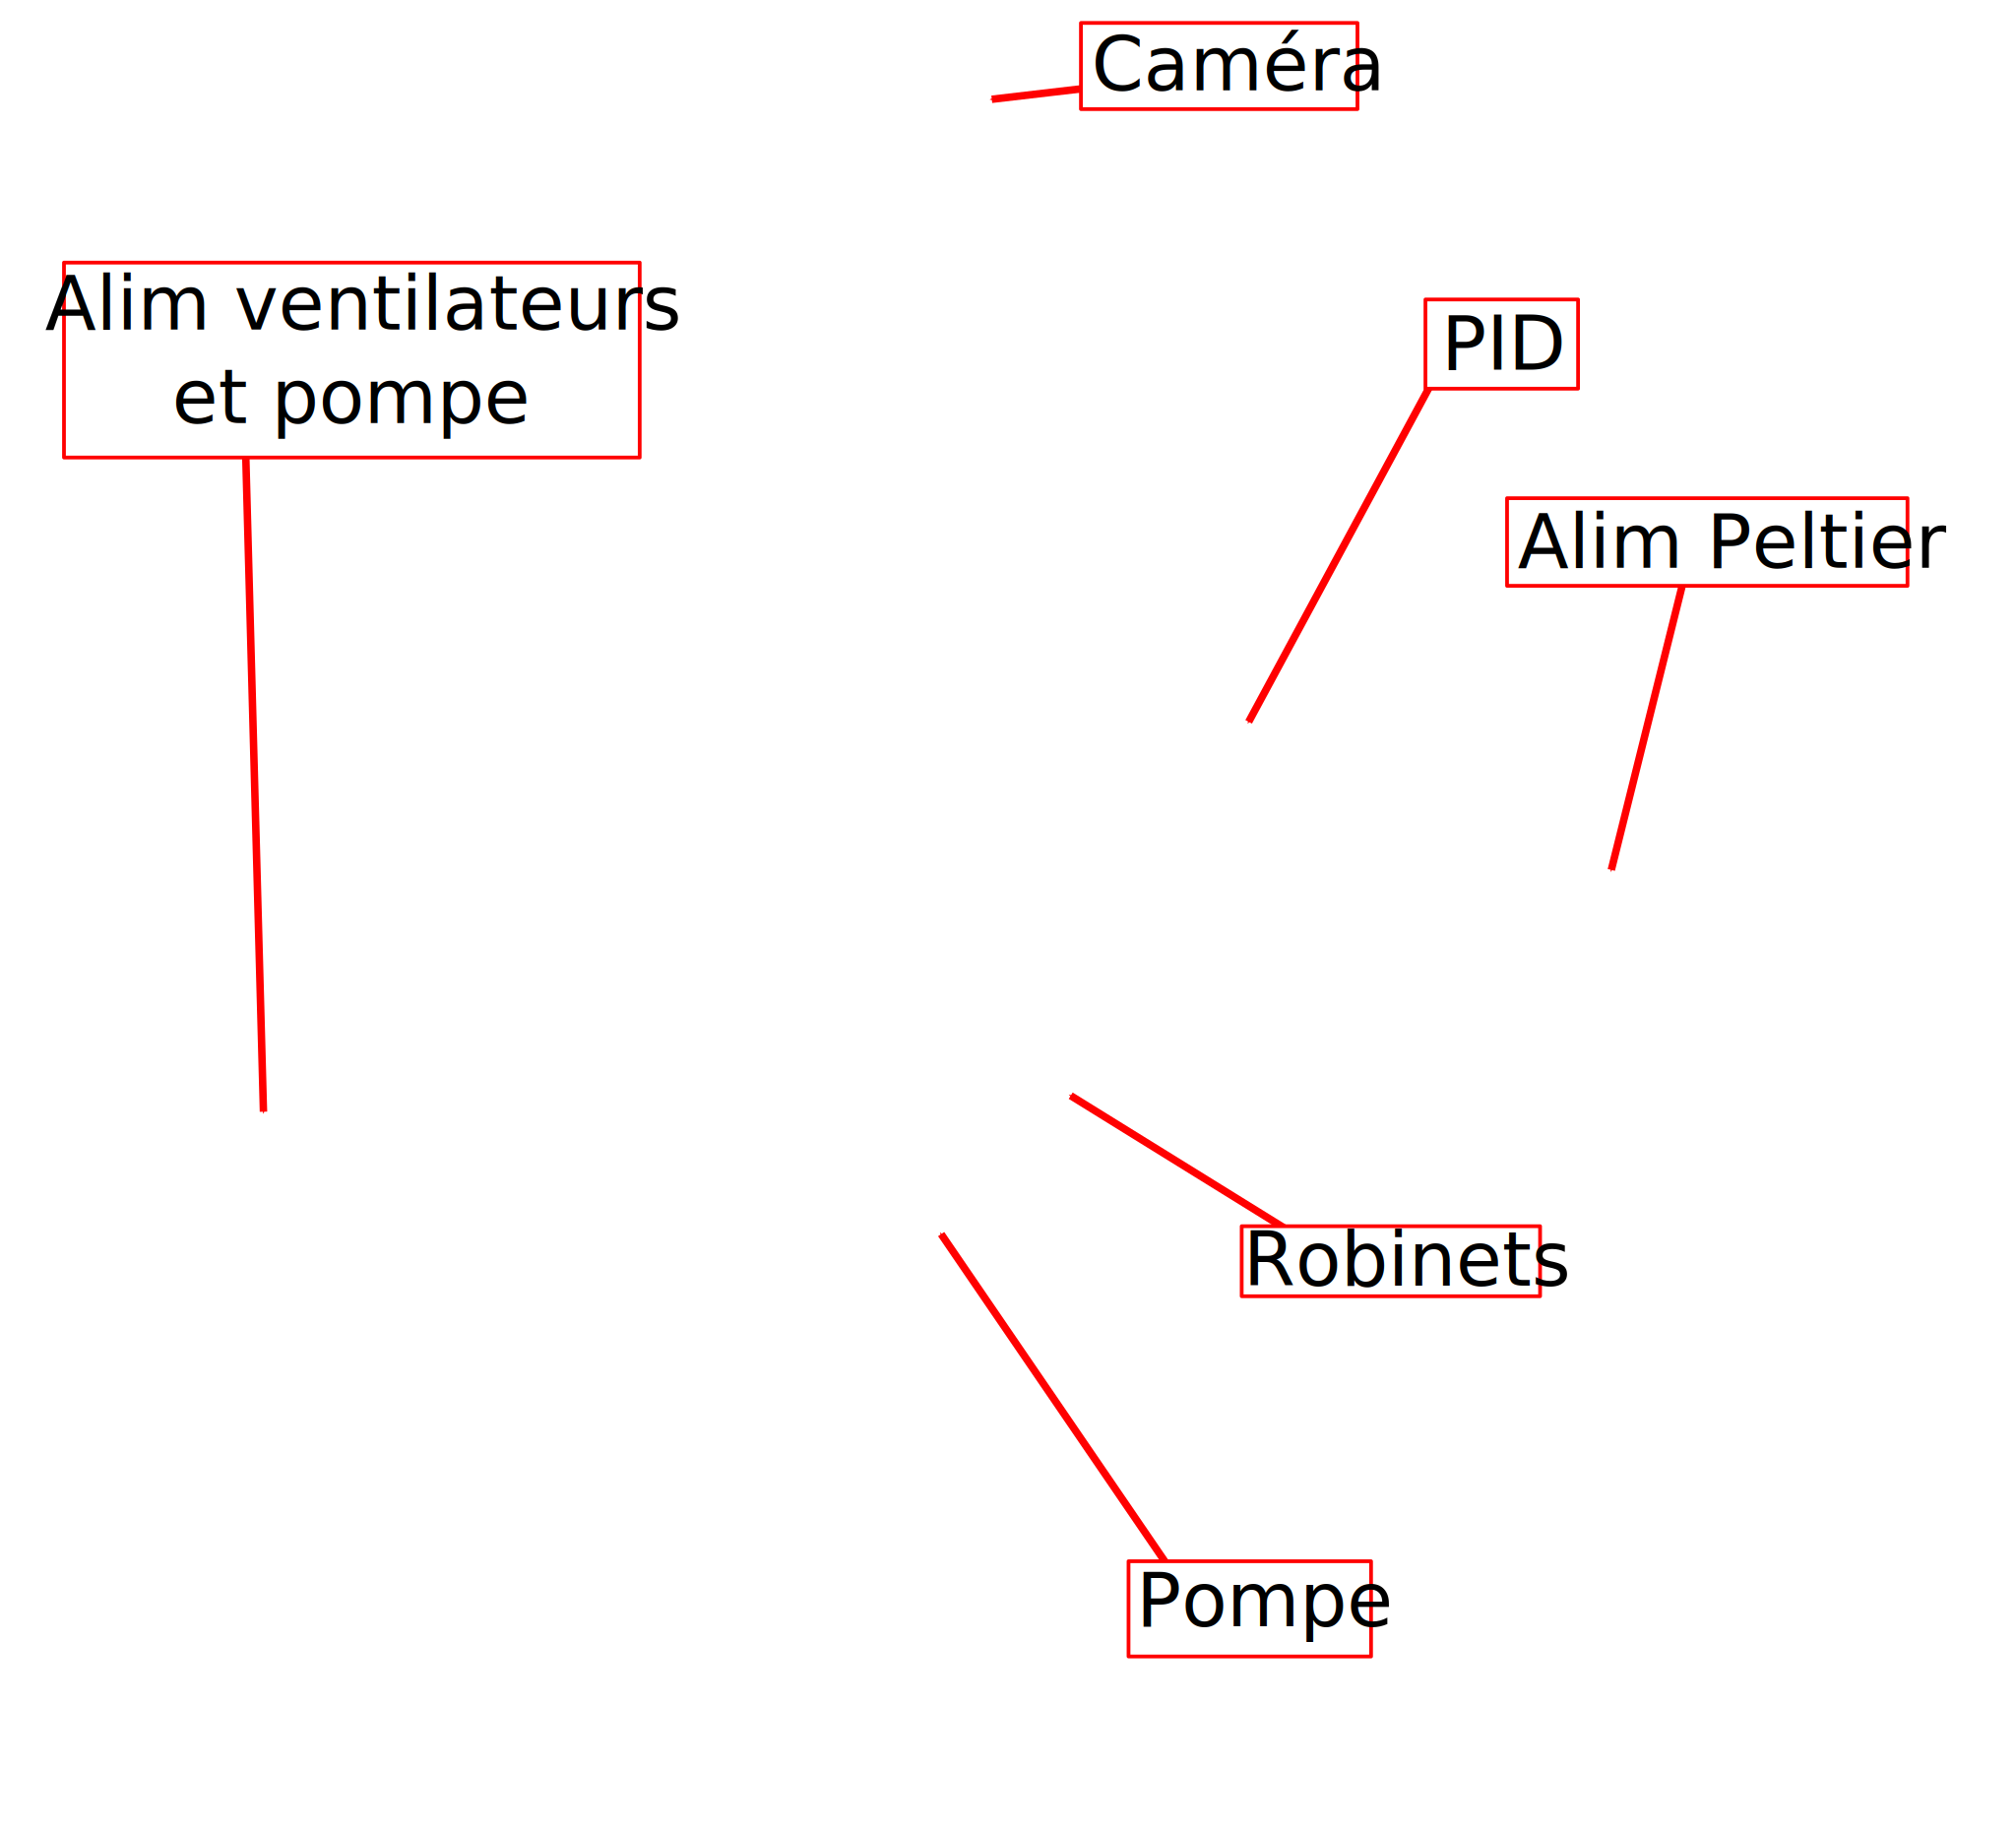
\includegraphics[width=1\columnwidth]{loin.pdf}
		\caption{Vue d'ensemble}
		\end{subfigure}
	~
		\begin{subfigure}[b]{0.43\textwidth}
		\centering
		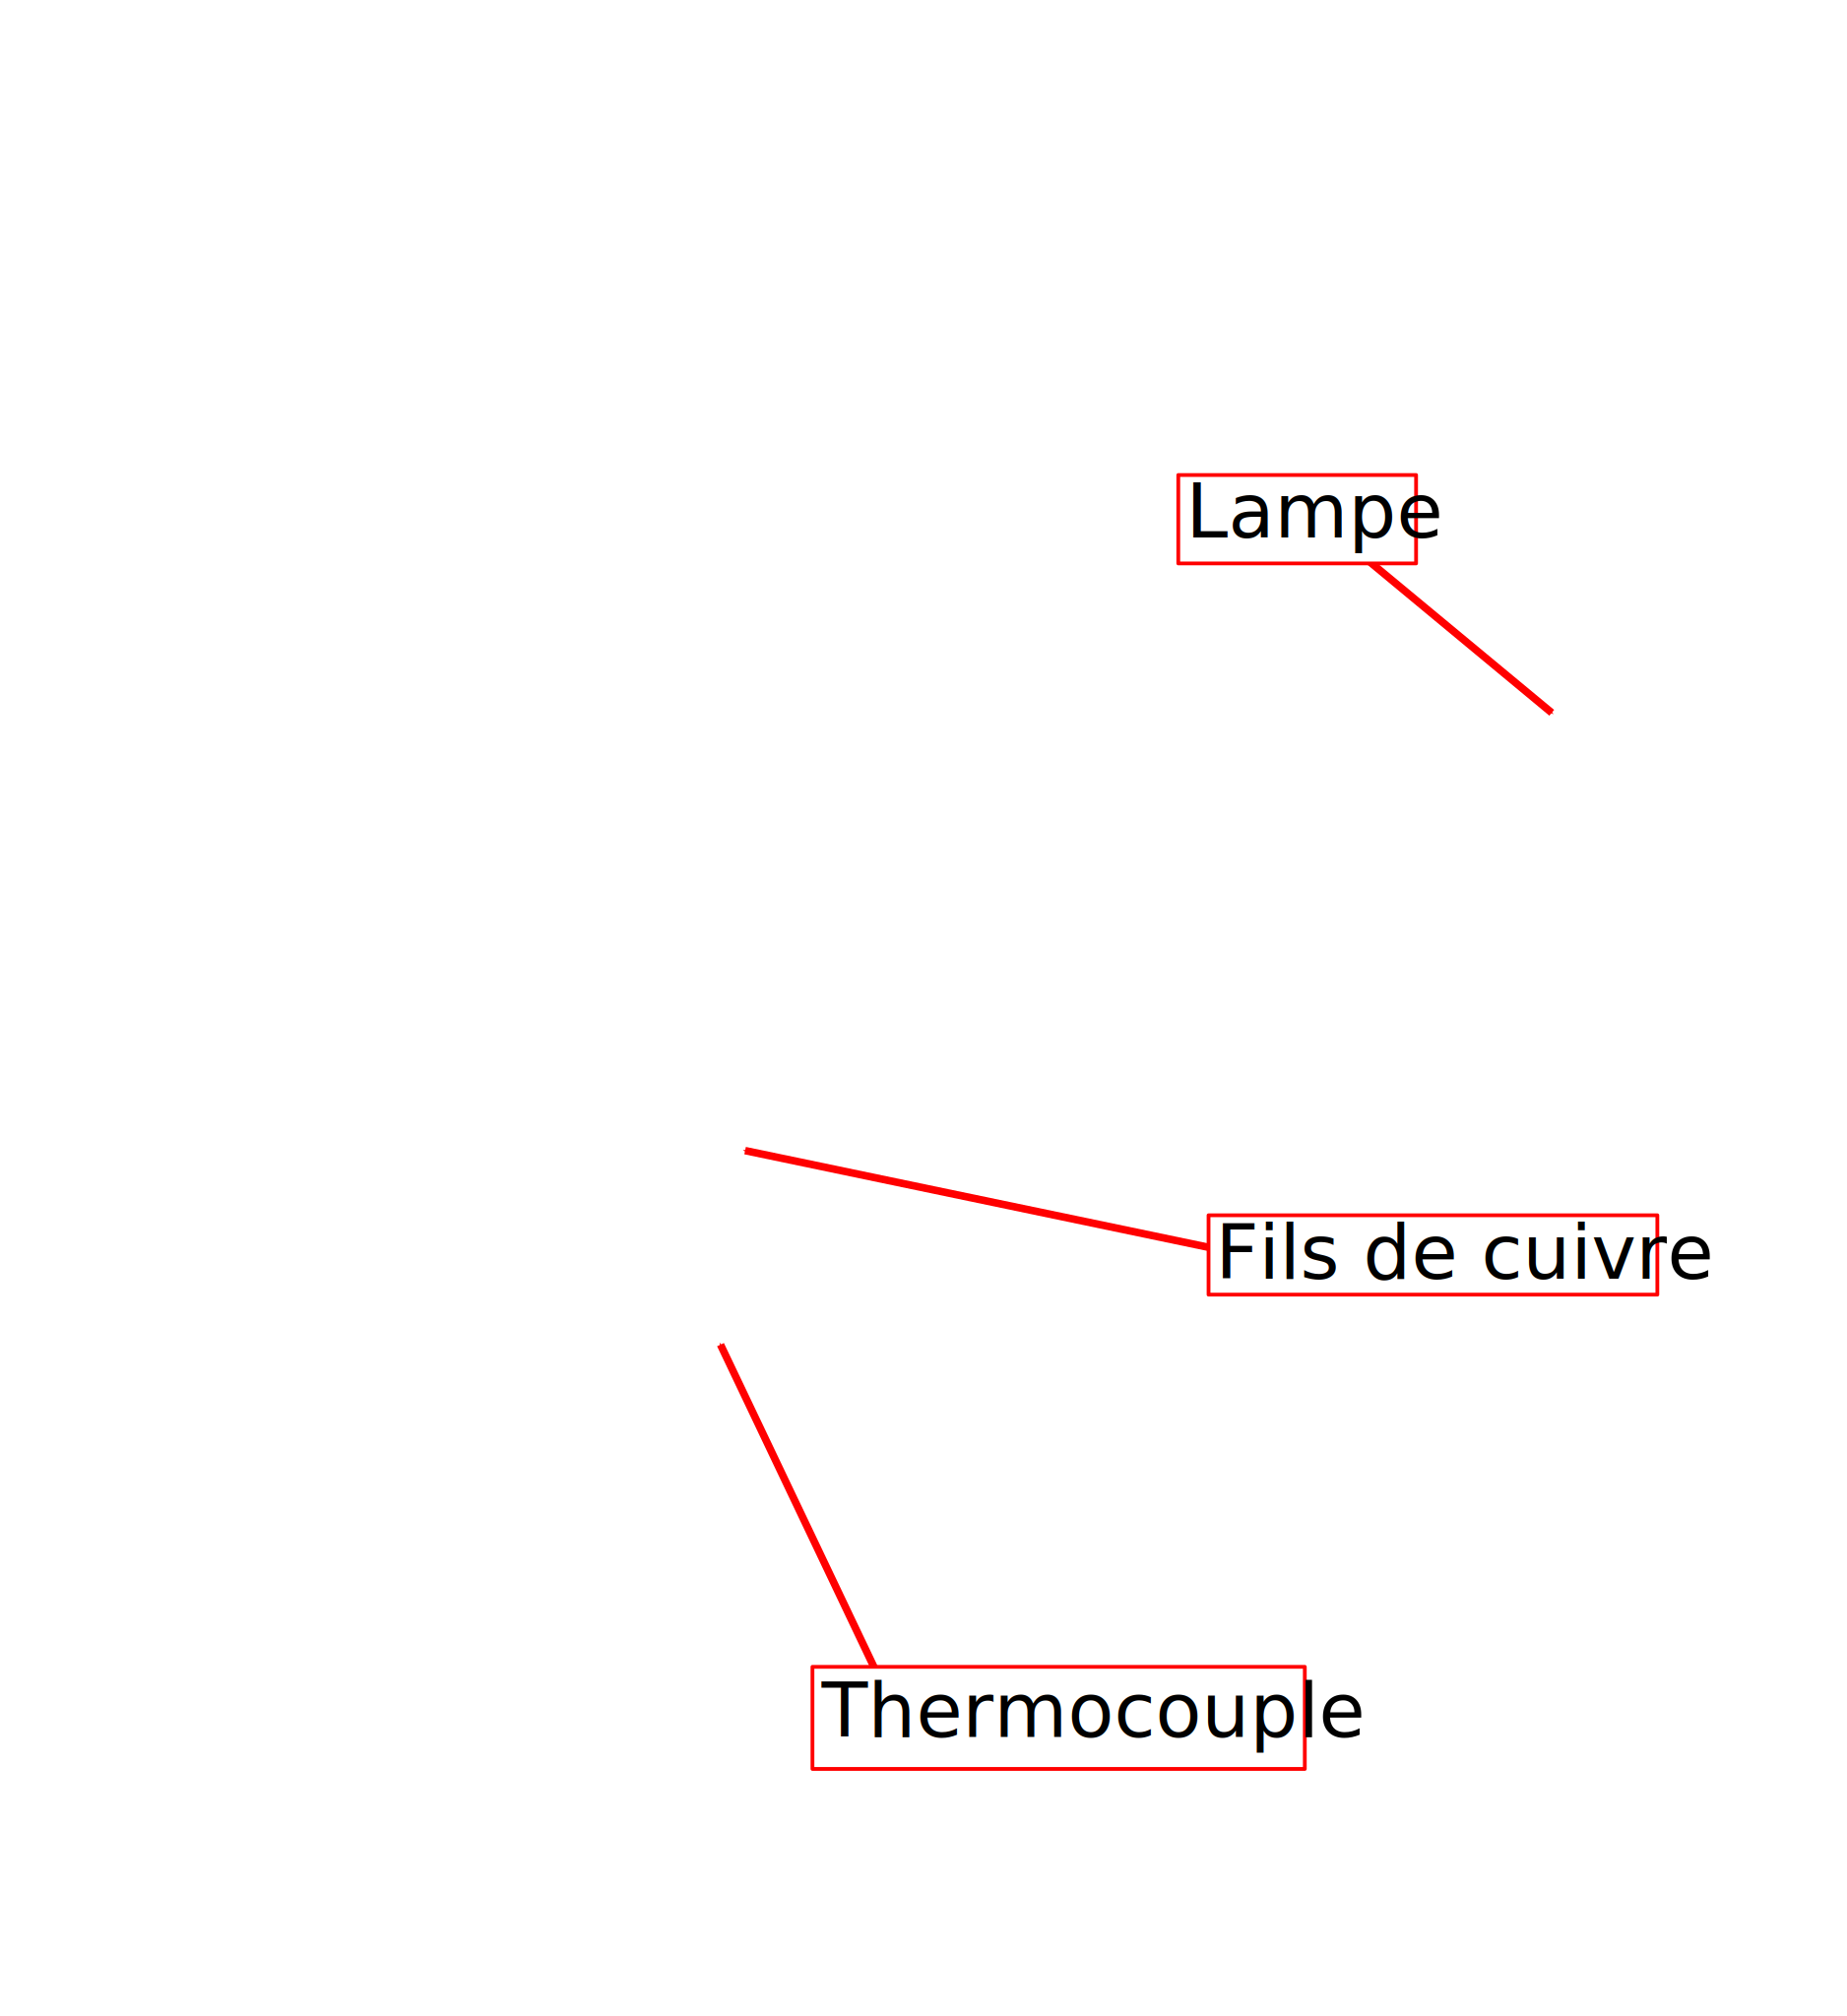
\includegraphics[width=1\columnwidth]{proche.pdf}
		\caption{Vue de proche}
		\end{subfigure}
	\end{figure}
	
	Le système de refroidissement est constitué de deux éléments Peltier branchés en série (max 5.5A) et d'un refroidissement liquide formé d'une pompe (12V) et de deux ventilateurs (12V) branchés en parallèle.
	
	L'alimentation des Peltier est contrôlée par un PID.

\section*{Marche à suivre}
	\begin{enumerate}
		%\item Chasser l'air (naturellement humide) qui est dans la chambre de travail en injectant de l'azote depuis la bouteille (gaz sec). Ou bien faire aspirer l'air avec une pompe.
		\item Fermer les deux petits robinets pour empêcher que des cristaux de glace ne se forment pendant la phase de refroidissement.
		\item Alimenter les ventilateurs et la pompe avec 12V.
		\item Régler la consigne de température sur le PID à l'aide des deux flèches oranges, puis enclencher l'alimentation de l'élément Peltier. Le courant de sortie de l'alimentation est contrôlé par le PID. 
		\item Attendre que la température soit atteinte.
		\item Laisser entrer de l'air (de l'humidité) dans la chambre de travail et observer la formation des cristaux de glace.
	\end{enumerate}

\end{document}
